\documentclass[a4paper,12pt,hidelinks]{report}

%%Pacchetti utili anche se non necessari

\usepackage{amsfonts}
\usepackage{amsmath}
\usepackage{latexsym}
\usepackage{tabularx}
\usepackage[italian]{babel}
\usepackage[bookmarks=true]{hyperref}
\usepackage{url}
% \usepackage{subfigure}
\usepackage{epstopdf}
\usepackage[utf8]{inputenc}
% \usepackage[utf8x]{inputenc}
\usepackage{listings}
\usepackage{graphicx}
%-------------------------------------------

\title{Progettazione sito web\\ ''B\&B La Vecchia Posta''}
\author{Daniele Di Pompeo \\mat. 226766}
% \annoaccademico{2013-2014}
\begin{document}
%   \begin{figure}%
% 	\includegraphics[scale=1.5,keepaspectratio=true]{img/vpLogo}%
% 	\centering
%   \end{figure}

\maketitle
\tableofcontents

%----------------------------------------------------
\begin{abstract}
In questo documento verranno descritti nel dettaglio tutti i requisiti funzionali e non funzionali individuati per la realizzazione del sito web del B\&B La Vecchia Posta.
Per la realizzazione del nuovo sito web sono state utilizzate le informazioni sul traffico dati utilizzando ``google analytics''. Sono stati presi in visione i siti web di altre strutture
locali e nazionali per rendere la versione 2.0 del sito del B\&B La Vecchia Posta una versione all'avanguardia utilizzando tutte le nuove tecniche del web 2.0.
\par Nella prima parte di questo documento si riporta una descrizione dell'attività del committente ponendo l'attenzione sui dati statici raccolti.
\par Nella seconda parte vengono descritti in maniera puntuale i requisiti funzionali per la realizzazione del nuovo sito web. Come framework di sviluppo verrà utilizzato ``beContent'' tool 
sviluppato dall'università dell'Aquila, del quale il sottoscritto è uno sviluppatore.
\end{abstract}

\chapter{Generalità}

\section{Il Committente}
Il B\&B La Vecchia Posta, inaugurato nell'Agosto del 2010 è situtato in Via Amiternum n 6 nel comune di Cagnano Amiterno, a pochi chilometri dal centro della città di L'Aquila.
Offre ai suoi clienti 6 spaziose camere tutte con bagno privato, ampio spazio verde di proprietà garantendo ai suoi clienti il massimo confort e relax. 
Si riporta una veduta aerea dell'area del B\&B per far rendere conto al lettore la posizione geografica e la conformazione dello spazio (fig.\ref{fig:bbArea}). 

\begin{figure}[h!]%
	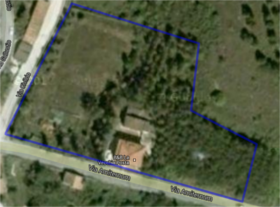
\includegraphics[width=0.6\textwidth,keepaspectratio=true]{img/bbArea1}
	\centering
	\caption{Veduta area del B\&B La Vecchia Posta}%
	\label{fig:bbArea}%
\end{figure}
Il B\&B è a conduzione familiare, il titolare, l'autore di questo documento, è aiutato dai genitori Emanuela e Nando, incuriositi nel conoscere nuove persone per impoarare usi e costumi di diversi luoghi.
Dall'analisi dei dati raccolti il sottoscritto si è reso conto che molta della pubblicità programmata su internet, tramite il servizio ``google adword'', non portava ai risultati attesi,
quindi è sorta la neccessità di aggiornare il sito web attuale.

\section{Situazione attuale}
Il B\&B La Vecchia Posta risulta essere titolare di un dominio web dall'URL www.vecchiaposta.it, al momento non sono stati previsti alias. 
\par Il sito web è stato realizzato nel 2010 dalla Fermenti Grafici, web agency aquilana, che a titolo di amicizia ha realizzato
il comparto grafico (logo, foto, template) ed ha fornito gratuitamente e momentaneamente l'hosting.
Ad oggi il sito web risulta essere completamente gestito dal sottoscritto ed è hostato dalla web farm ARUBA.
\par Sin dalla sua prima versione il sito web del B\&B è stato realizzato utilizzando WordPress, uno dei più famosi CMS nel mondo del web e sono stati installati alcuni plug-in per fornire al sito alcune funzionalità di cui il committente aveva bisogno.

\subsection{Aspetti rilevanti del sito}
Da interviste effettuate sui clienti del B\&B risulta essere di gradevole impatto il sito, grazie ad una grafica curata minuziosamente.
sempre ascoltando i parari di terzi il sito web risulta essere di facile navigazione offrendo informazioni dettagliate per le singole pagine.
\subsection{Principali pregi}
L'intero sito web non ha oggetti in flash, che renderebbero il sito non navigabile dadispositivi mobile.
La homePage effettua 86 HTTP Request per un peso complessivo di circa 60Kb scaricabili in circa 3 secondi con una connessione a banda larga di velocità media (4Mb)
La struttura dell'intero sito + sempre coerente fornendo uno spazio per l'immagine principale della pagina, che pèuò anche essere uno slider, e dello spazio binanco per il testo rendendo la lettura gradevole
non affaticando gli occhi del lettore.
\subsection{Principali difetti}
I principali difetti sono legati dalla difficoltà nel raggiungere il collegamento per effettuare una richiesta di prenotazione, accessibile solamente tramite la barra di nabigazione o
tramite il link nascosto dietro il testo dell'ultimo articolo inserito, che nel nostro caso sono le ultime news. Questo è visibile anche dai dati raccolti da google analytics che mostrano come un utente medio
resti sulla home page poco meno di 2 minuti e abbandona il sito prima di inviare una richiesta di prenotazione. Evidente dal fatto che il link prenota non risulta mai essere cliccato.

\begin{figure}[h!]%
	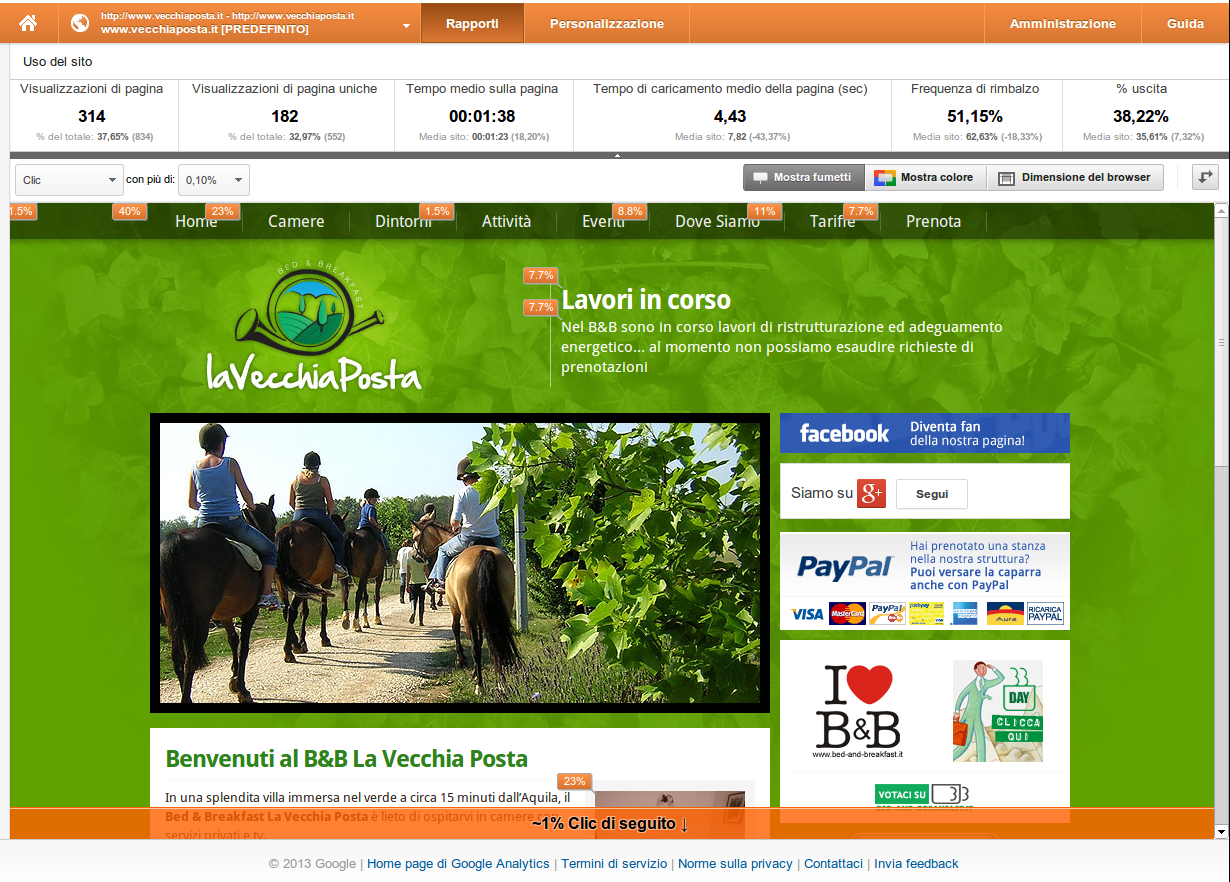
\includegraphics[width=0.95\textwidth,keepaspectratio=true]{img/googleAnalyticsDoc1}
	\centering
	\caption{Dati Google Analitycs Home Page}%
	\label{fig:googleHomePage}%
\end{figure}
Dall'immagine {fig.\ref{fig:googleHomePage}} postata risulta evidente che la barra di navigazione posta sopra il logo rende difficoltosa all'utente medio comprendere quale sia il vero link alla homePage, si notano alcuni click sullo spazio negativo della
barra di navigazione (più del 40\% degli utenti).
Non permette la modifica della grandezzzqa del font, non permettendo una facile navigazione a persone ipovedenti.

\section{Obiettivi generali del nuovo sito}
La nuova versione del sito web dovrà eliminare queste problematiche, invogliando gli utenti ad inviare più richieste di prenotazioni inserendo nella parte ``sopra la piega'' un link
al forma di prenotazione di prenotazione.
Per il comparto grafico si è scelta di comprare un tema html dal sito ThemeForest.com, con le funzionalità richieste.
Il nuovo sito inoltre, nella versione base dovrà fornire le informazioni ad oggi presenti nella versione attuale migliorando la navigabilità spostando la barra di navigazione al di sotto 
del logo del B\&B.
\par L'home page del sito dovrà restare leggera e non dovrà prevedere nessuna funzionalità in flash, che la renderebbe inaccessibile dai dispositivi mobile.
L'intento è di fornire ``\textit{sopra la piega}`` tutte le informazioni utili come:
\begin{itemize}
 \item collegamento all'home page al click sul logo
 \item barra di navigazione al di sotto del logo
 \item slider di immagini
 \item form per la richiesta di disponibilità
 \item preview dell'offerta attiva
\end{itemize}
\par Inoltre il nuovo sito dovrà essere ''responsive'' garantendo la completa compatibilità con i maggiori device che ad oggi accedono ad internet.
\\In particolare:
\begin{itemize}
 \item 1200px Desktop
 \item 1024px iPad landscape and netbook
 \item 768px 7inch tablet
 \item 368px mobile phone
\end{itemize}
Prendendo come risoluzione base 1200px essendo circa il 90\% degli utenti ad utilizzarla \footnote{Fonte \url{http://www.w3schools.com/browsers/browsers_display.asp}}
ed inoltre facendo attenzione alla compatibilità fra i differenti browser (chrome, firefox, safari, explorer ed opera).

\section{Utenti}
Dall'analisi effettuata risultano essere stati individuati tre categorie di utenti:
\begin{itemize}
 \item L'amministratore
 \item L'utente occasionale (utente che raggiunge il sitoweb involontariamente) (aka \textit{Utente})
 \item Il cliente (navigatore di internet che effettua una richiesta di prenotazione)
\end{itemize}

\begin{center}
  \begin{tabular}{||m{3cm}||m{4cm}|m{1,5cm}||m{4cm}|m{1,5cm}||}
    \hline
      \textbf{Categoria di utenti} & \textbf{Bisogni principali degli utenti in relazione al sito} & Priorità & \textbf{Obiettivi del committente} & Priorità \\
    \hline
      Amministratore & mantenere aggiornarnate le informazioni presenti sul sito & alta & fornire all'amministratore le informazioni aggiornate da inserire nel sito web & alta\\
    \hline
      Utente & reperire le informazioni di contatto, prendere visione della struttura
	     & alta, alta
	     & impressionare l'utente casuale invogliando ad effettuare una prenotazione,  & alta\\
    \hline  
      Cliente & reperire informazioni di contatto, visionare il tariffario, effettuare una richiesta di prenotazione & alta, media, alta & mantere ottimi rapporti con
      il cliente abitudinario, invogliare il ``passaparola'' dei clienti & alta, alta\\
    \hline
  \end{tabular}
\end{center}
\subsection{Profilo degli utenti}
  \begin{itemize}
   \item \textbf{Cliente}: sono i navigatori di internet che cercando una destinazione per le proprie vacanze si sono imbattuti sul sito web della struttura e hanno la volotà di inviare 
   una richiesta di disponibilità. Rientrano in questa categoria di utenza anche i clienti ``storici'' del B\&B avendo già soggiornato nella struttura in un'altra occasione.
   \item \textbf{Utente}: sono i navigatori di internet definiti come i visitatori di rimbalzo, ovvero quegli utenti di internet che non volendo sono giunti sul sito internet del B\&B. 
   Su questi utenti che il titolare vorrebbe invogliare a fare una richiesta di disponibilità.
   \end{itemize}

\section{Scenari d'uso}
\par
\begin{itemize}
 \item [Cliente] inserire qui una storia
 \item [Utente] inserire qui una storia
\end{itemize}

\section{Posizionamento competitivo}
Particolare attenzione verrà posta nel posizionamento competitivo il sito web della struttura. Per ottenere un risutlatao di pregio sono stati analizzati i siti web di altre strutture
locali ma anche di strutture nazionali, delle maggiori località turistiche, per catturare quelle funzionalità che potevano sfuggire ma che risultano essere utili.
\par I siti web locali analizzati sono stati:
\begin{itemize}
 \item B\&B Camaga
 \item B\&B Oasi nel Vetoio
 \item B\&B Grace
\end{itemize}
mentre per i siti extra-regione sono stati analizzati:
\begin{itemize}
 \item Il giglio binaco (Sorrento)
 \item Soggiorno Pezzati (Firenze)
 \item Il Melograno (Muro Leccese)
\end{itemize}
\par Per il nuovo sito si intende posizionarlo nei primissimi posti dei motori di ricerca (google, bing, yahoo) cercando di migliorare l'inidicizzazione.



%----------------------------------------------------

\chapter{Requisiti del sito}

\section{Requisiti di architettura}

\section{Requisiti di comunicazione}

\section{Requisiti funzionali}
	\subsection{Casi d'uso}
	\subsection{Base di dati}
	\subsection{Sicurezza e privacy}

\section{Requisiti di contenuto}

\section{Requisiti di gestione}
	\subsection{Infrastruttura per l'esercizio del sito}
	\subsection{Gestione dei sistemi}
	\subsection{Gestione del sito}
	\subsection{Gestione dei contenuti}
	\subsection{Getione degli utenti}

\section{Requisiti di accessibilità}
	\subsection{Prestazioni}
	\subsection{Reperibilità}
	\subsection{Compatibilità con i browser}
	\subsection{Accessibilità da parte di utenti disabili}

\section{Requisiti di usabilità}

\section{Glossario}

%----------------------------------------------------

\chapter{Requisiti di gestione progetto}

\section{Tempi e risorse}
\section{Gruppo di progetto}
\section{Responsabilità del committente}
\section{Documentazione prevista}
\section{Verifiche e convalide}
\section{Consegna finale e pubblicazione del sito}
\section{Ambiente di sviluppo}
\section{Altri requisiti}
\section{Analisi dei rischi}


\end{document}